A frequent issue with localization when using cost effecitve GPS sensors is a radial drift component that cause inaccurate location readings. Managing this issue boiled down to separating the problem into two cases: 1) anchor initialization, then 2) dynamic localization. 

Anchor initialization uses trianglulation and vigorous averaging to mark a global reference point. The goal is to, through set number of iterations $I_{max}$, create a anchor node that exists at an agreed upon new origin of each agents virtual map. Initial experiments placed rovers at locations (0,1), (1,1), (1, 0), (-1,0), (-1,-1), and (1,-1) and then based on simulated GPS drift of each rover approximated the central anchor node. Figure~\ref{fig:init} displays promising results of this experiment over 1000 iterations.

\begin{figure} 
	\centering
	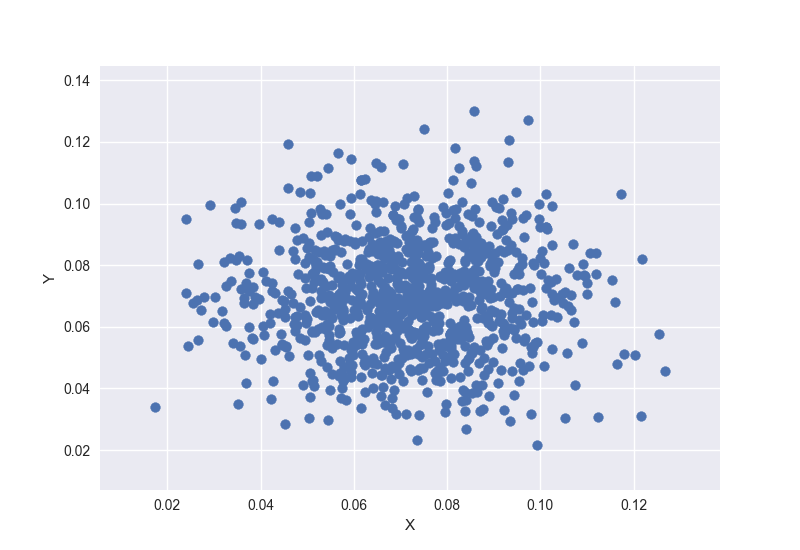
\includegraphics[scale=0.4]{initialization}
	\caption{Possible anchor node positions, between rovers (1000 iterations).}
	\label{fig:init}
\end{figure}

If each point in the figure is an agreed upon global reference point, then the graph suggests that our initialization algorithm is percise, but not entirely accurate. 


Modeled below is graph of the localization of a single rover. The ideal path can be seen in black, originating at the origin (0,0) and traversing to point (1,3). 

\begin{figure} 
	\centering
	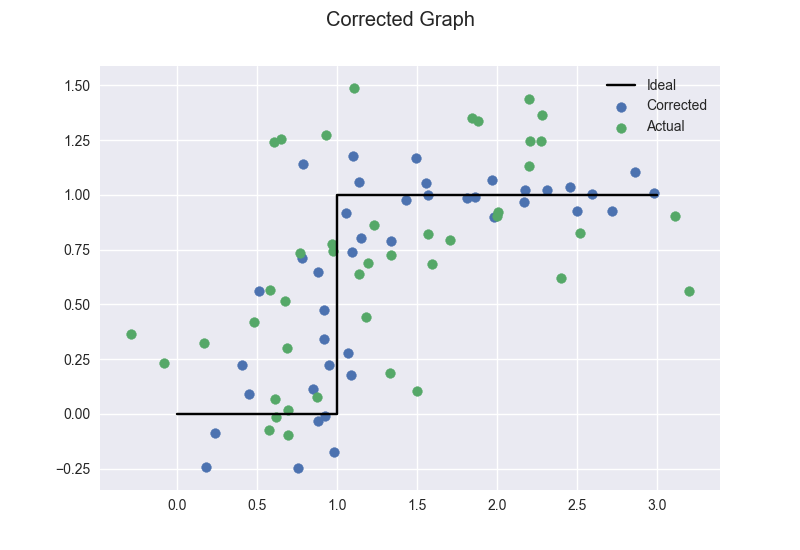
\includegraphics[scale=0.5]{localization}
	\caption{Dynamics localization as rover travels from (0,0) to (3,1).}
	\label{fig:dynamic}
\end{figure}


\begin{itemize}
	\item Mean Square Error = 0.0067 
	\item $R^2$ Regression Score = 0.964 
\end{itemize}
